\documentclass[times]{article}

\usepackage{graphicx}
\usepackage{float}
\usepackage{placeins}
\usepackage[none]{hyphenat}
\usepackage{amsmath}
\usepackage[us]{datetime}
\usepackage[explicit]{titlesec}
\titleformat{\section}{\normalfont}{}{0em}{\textbf{\large Problem  \thesection}\  \normalsize #1}
\begin{document}
	\title{CS 5800 Distributed OS - Spring 2017 \\ Homework 3}
	\author{Josh Herman \\ Dalton Cole \\ Neil Blood}
	\date{\formatdate{7}{3}{2017}}
	\maketitle

	\section{How to define causality in a distributed system?}
		Causality helps identify sequential and concurrent events without using physical clocks. If \textbf{a}, \textbf{b} are two events in a single process \textbf{P}, and the time of \textbf{a} is less than the time of \textbf{b} then \textbf{a} $\prec$ \textbf{b}. If \textbf{a} = sending a message, and \textbf{b} = receipt of that message, then \textbf{a} $\prec$ \textbf{b}. \textbf{a} $\prec$ \textbf{b} $\wedge$ \textbf{b} $\prec$ \textbf{c} $\Rightarrow$ \textbf{a} $\prec$ \textbf{c}.
	
	\section{Can the simple counter based logical clock be used to detect causality? Why or why not?}%Problem2
		No because the logical clocks might not be in sync so even if process $b$ happened before process $a$, the logical clock of $b$ could be larger than $a$. Even if they are in sync process $a$ could be unrelated to process $b$ making them having concurrency, absence of causal order. Therefore $LC(a)<LC(b)$ does not imply $a \prec b$.


	\section{According to Figure 1, there are three processes and their local events are denoted by $a, b,...,m$. Provide the vector clock values for these events.}%Problem 3}

	\begin{figure}[H]
		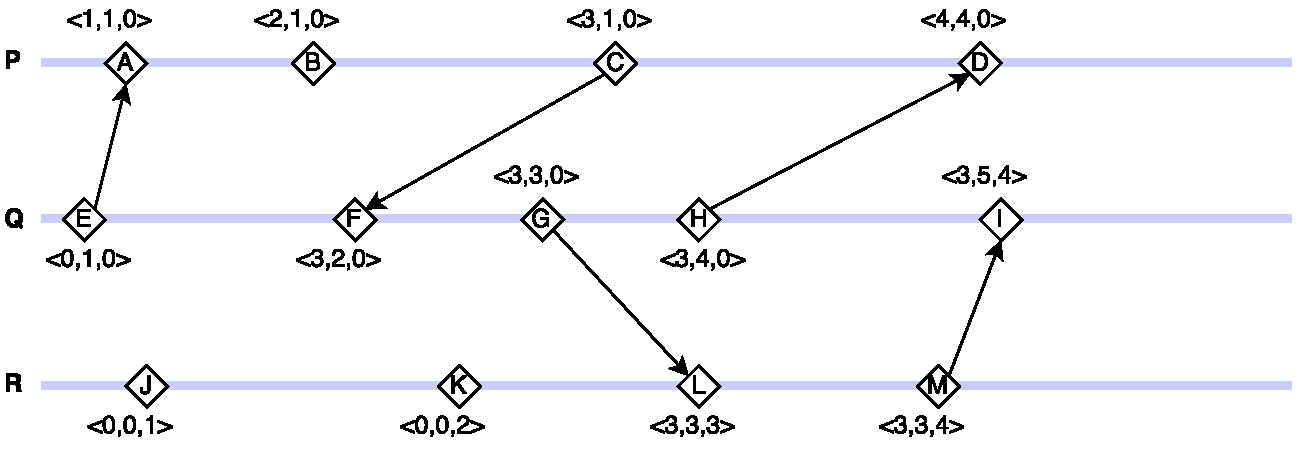
\includegraphics[width=\linewidth]{CS5800HW3.pdf}
		\caption{Events related to three processes: P, Q and R}
	\end{figure}

	

	\section{Regarding the Lamport and Melliar-Smith's internal clock synchronization algorithm, using induction, prove that the maximum difference between the averages computed by two non-faulty modes is $\dfrac{3t \delta}{n}$, where $t$ is the number of faulty clocks and $n$ is the total number of clocks in the system. You can assume $t < n-1$.}%Problem 4}
		Base Case: $n=3 \Rightarrow t < 2$\\
		$i: \dfrac{c+(c-\delta) + (c+ \delta) }{n}=\dfrac{c+(c-\delta) + (c+ \delta) }{3}=c$\\
		$j: \dfrac{c+(c-\delta) + (c- 2\delta) }{n}=\dfrac{c+(c-\delta) + (c-2 \delta) }{3}=c-\delta$\\
		$i-j:c-(c-\delta)=\dfrac{3t\delta}{n}$\\
		$\delta=\dfrac{3\delta}{3}=\delta$\\
		Assume true for $n=k$\\
		Prove true for $n=k+1 \Rightarrow t<k+1-1\Rightarrow  t<k $\\
		For the maximum possible difference in averages $t=k-1$ and the number of good clocks would be 2.\\
		$i: \dfrac{c+(c-\delta)+t(c+\delta)}{n}=\dfrac{c+(c-\delta)+(k-1)(c+\delta)}{k+1}$\\
		$j: \dfrac{c+(c-\delta)+t(c-2\delta)}{n}=\dfrac{c+(c-\delta)+(k-1)(c-2\delta)}{k+1}$\\
		$i-j=\dfrac{c+(c-\delta)+(k-1)(c+\delta)}{k+1}-\dfrac{c+(c-\delta)+(k-1)(c-2\delta)}{k+1}$\\
		$i-j=\dfrac{(k-1)((c+\delta)-(c-2\delta))}{k+1}=\dfrac{(k-1)3\delta}{k+1}$\\
		$\dfrac{3t\delta}{n}=\dfrac{3(k-1)\delta}{k+1}$\\
		$i-j=\dfrac{3t\delta}{n}$\\
		Therefore by proof by induction the maximum difference is $\dfrac{3t\delta}{n}$, where $t$ is the number of faulty clocks and $n$ is the total number of clocks in the system.


	\section{Refer to slide \#5-6 of "lec6.pdf", what is the fairness property? Does the fairness property hold? Why or why not?}%Problem 5}
	The fairness property in this scenario would be that processes with a lower time stamp will be able to enter the critical section first. \\
	The fairness property does NOT hold because the queue adds requests as they come in with no priority on them. A possible solution would be to implement a priority queue instead of a normal queue that was sorted based on smallest time stamp. \\
	

	
	
		
\end{document}